% CircusTent Section

CircusTent

\begin{figure*}[!t]
\centering
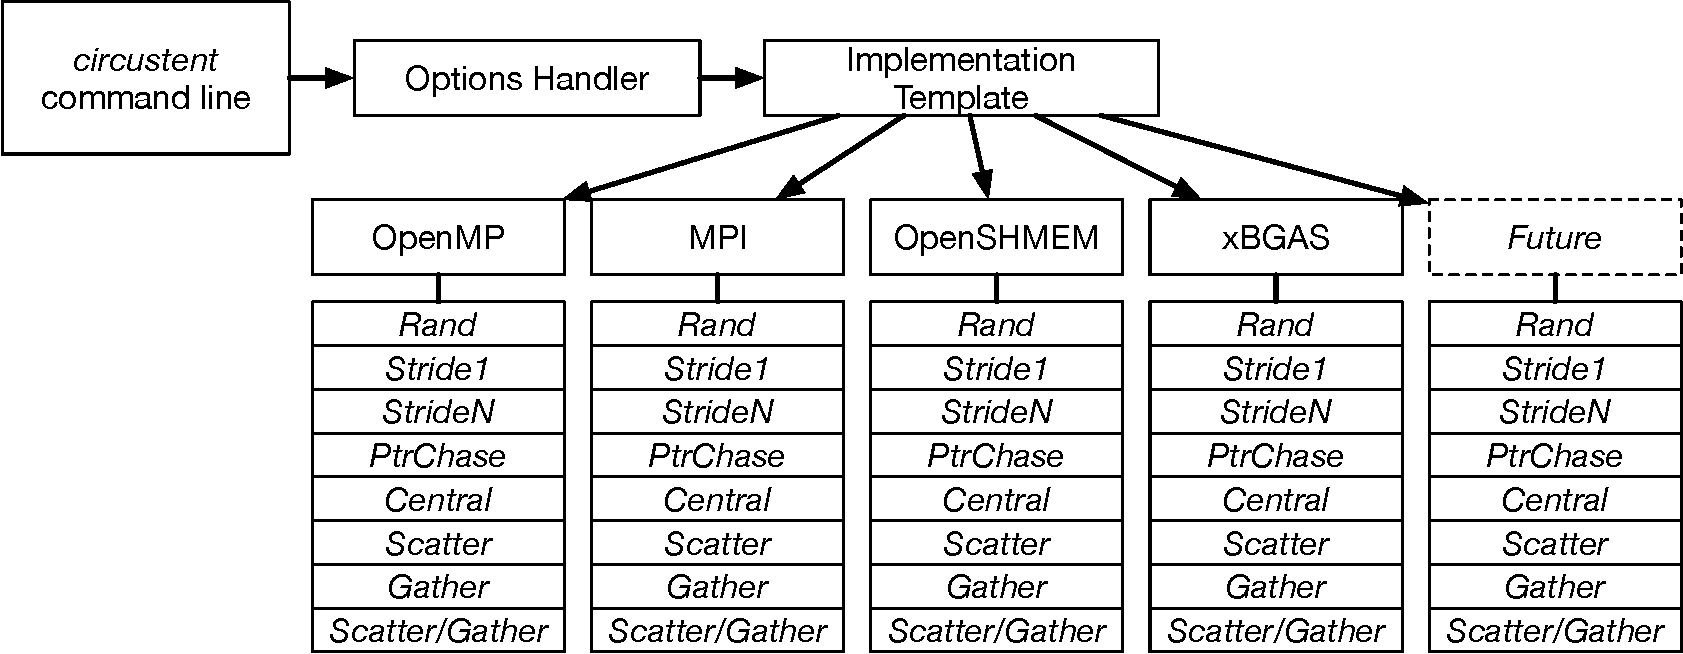
\includegraphics[width=5in]{figures/arch.pdf}
\caption{CircusTent Architecture}
\label{fig:ct_arch}
\end{figure*}

\subsection{Benchmark Overview}
\label{subsec:benchmark_overview}

\subsection{Programming Models}
\label{subsec:programming_models}

\subsection{Algorithms}
\label{subsec:algorithms}

The CircusTent infrastructure contains eight individual benchmark kernels.
Each kernel is described in terms of a generic atomic operation, or \textit{AMO}.  
However, each kernel may be implemented using any platform-supported atomic operations.
In the case of this study, we utilize atomic \textit{Add} and atomic \textit{Compare-and-Swap} (CAS) operations to implement each kernel, respectively.  

The first kernel is a basic random access kernel (Algorithm~\ref{alg:1}).
The kernel allocates two array structures.
The \texttt{VAL} array contains a series of values.
The \texttt{IDX} array contains a series of valid indices within the scope of the \texttt{VAL} array.
Prior to the execution of the kernel, the indices are randomly selected and written to the \texttt{IDX} array using a linear congruential randomizer.
For each iteration of the loop, a single \texttt{VAL} array entry is updated using an atomic operation.
In this manner, the random access kernel contains one memory load (\texttt{IDX[i]}) and one atomic operation for each iteration of the loop.
The goal of this kernel is to observe the performance of atomic operations when the platform has a limited ability to cache data for subsequent iterations.  

\begin{algorithm}
\SetAlgoLined
\For{$i\gets0$ \KwTo $iters$ \KwBy $1$}{
AMO(VAL[IDX[i]])
}
\caption{Random Access Kernel}
\label{alg:1}
\end{algorithm}

The second kernel encapsulates a simple, stride-1 kernel (Algorithm~\ref{alg:2}).  
The kernel allocates a single array (\texttt{VAL}) that contains a series of values.  
For each iteration of the loop, the kernel updates a single value in the array in linear fashion using a single atomic operation.
In this manner, a platform may utilize data prefetching and/or caching in order to optimize the access to data members in this kernel in an optimal manner similar in form to dense vectors or matrices.  

\begin{algorithm}
\SetAlgoLined
\For{$i\gets0$ \KwTo $iters$ \KwBy $1$}{
AMO(VAL[i])
}
\caption{Stride-1 Kernel}
\label{alg:2}
\end{algorithm}

The third kernel is similar in form to the second kernel.
In this kernel, we utilize the same \texttt{VAL} array structure as mentioned above, but we permit the user to define the unit stride by which we access the array (Algorithm~\ref{alg:3}).  
For example, if the user seeks to determine what the raw memory bandwidth is of parallel atomics by forcing every access to induce a cache line miss, the stride-n kernel can accomplish this.
Further, for each parallel PE participating in the kernel execution, the starting index is at least \textit{iters} distance from the previous PE. 

\begin{algorithm}
\SetAlgoLined
\For{$i\gets0$ \KwTo $iters$ \KwBy $stride$}{
AMO(VAL[i])
}
\caption{Stride-N Kernel}
\label{alg:3}
\end{algorithm}

The fourth kernel included in the CircusTent suite is a pointer chasing kernel (Algorithm~\ref{alg:4}).
Similar to the random access kernel, this kernel makes use of an \texttt{IDX} array.
In this case, however, each preassigned random index within the array corresponds to another element of \texttt{IDX}.
Each PE begins the kernel loop by performing an atomic operation to an array location, \texttt{start}, determined using the PE's rank identifier.
For each subsequent iteration, the executed atomic operation is directly dependent on the index determined in the previous repetition.
This kernel therefore replicates the irregular memory access patterns common to many applications that utilize linked data structures such as graphs.

\begin{algorithm}
\SetAlgoLined
\For{$i\gets0$ \KwTo $iters$ \KwBy $1$}{
start = AMO(IDX[start])
}
\caption{Pointer Chase Kernel}
\label{alg:4}
\end{algorithm}

The fifth kernel is unique among those included in the CircusTent suite.
Rather than emulate a particular memory access pattern, the Central kernel is designed to measure performance in a worst case scenario (Algorithm~\ref{alg:5}).
Within each iteration of this kernel, every active PE performs an atomic operation to the same shared memory location, given by \texttt{VAL[0]}.
As a result, these accesses become serialized and performance quickly plateaus as the level of contention rises.
Depending on the underlying architecture, this behavior can also severely tax the cache hierarchy and associated interconnects.
For distributed shared memory systems, it also stresses the network interconnect.
Given the above, this kernel can be used to estimate minimum performance for applications that feature frequent memory hot spots.

\begin{algorithm}
\SetAlgoLined
\For{$i\gets0$ \KwTo $iters$ \KwBy $1$}{
AMO(VAL[0])
}
\caption{Central Kernel}
\label{alg:5}
\end{algorithm}

The sixth kernel replicates the scatter memory access pattern found in many modern HPC applications.
Herein, the \texttt{VAL} and \texttt{IDX} arrays are constructed as in the random access kernel.
In contrast to the previous kernels, this kernel performs multiple atomic operations during each of its iterations (Algorithm~\ref{alg:6}).
\todo[inline]{Finish scatter description}
\todo[inline]{Add sentence about scatter applications/use cases}

\begin{algorithm}
\SetAlgoLined
\For{$i\gets0$ \KwTo $iters$ \KwBy $1$}{
dest = AMO(IDX[i+1])\\
val = AMO(VAL[i])\\
AMO(VAL[dest], val) // VAL[dest] = val
}
\caption{Scatter Kernel}
\label{alg:6}
\end{algorithm}

Gather kernel...
\todo[inline]{Add sentence about gather applications/use cases}

\begin{algorithm}
\SetAlgoLined
\For{$i\gets0$ \KwTo $iters$ \KwBy $1$}{
dest = AMO(IDX[i+1])\\
val = AMO(VAL[dest])\\
AMO(VAL[i], val) // VAL[i] = val
}
\caption{Gather Kernel}
\label{alg:7}
\end{algorithm}

SG kernel...
\todo[inline]{Add sentence about sg applications/use cases}

\begin{algorithm}
\SetAlgoLined
\For{$i\gets0$ \KwTo $iters$ \KwBy $1$}{
src = AMO(IDX[i])\\
dest = AMO(IDX[i+1])\\
val = AMO(VAL[src])\\
AMO(VAL[dest], val) // VAL[dest] = val
}
\caption{Scatter/Gather Kernel}
\label{alg:8}
\end{algorithm}

We summarize the number of atomic operations required to perform each kernel in Table~\ref{tab:amodistro}.
However, this may vary depending upon how each platform implements a respective atomic operation.
The CircusTent implementation infrastructure supports the ability to override these defaults for each platform/programming model.    

\begin{table}
  \caption{Atomic Operation Distribution}
  \label{tab:amodistro}
  \begin{tabular}{cc}
    \toprule
    Benchmark&AMOs Per Iteration\\
    \midrule
   Rand & 1\\
   Stride-1 & 1\\
   Stride-N & 1\\
   Pointer Chase & 1\\
   Central & 1\\
   Scatter & 3\\
   Gather & 3\\
   Scatter/Gather & 4\\
  \bottomrule
\end{tabular}
\end{table}

\subsection{Normalizing the Results}
\label{subsec:normalizingtheresults}

Given the native extensibility of CircusTent to support a multitude of programming models and platforms, we seek to develop a normalized metric such that we can compare results across platforms and differing degrees of execution parallelism.
For this, we introduce the \textit{GAMs} metric.  

The \textit{GAMs}, or \textit{billions of atomic operations per second}, metric encapsulates the number of parallel execution elements (\textit{PEs}), the atomic operation algorithmic complexity, and the wall clock execution time in a single metric.
As we see in Equation~\ref{eq:gams}, the metric is a ratio of the total number of atomic operations executed for all parallel parallel execution elements (in billions) across all iterations and the wall clock execution time.
The atomic operation algorithmic complexity is the total number of atomic operations required for a single \textit{PE} to execute a single iteration of the target CircusTent kernel.
This is equivalent to the \textit{AMOs Per Iteration} column in Table~\ref{tab:amodistro}.  

\begin{equation}
\label{eq:gams}
  GAMs = \frac{(PEs \times Iters \times AMOs\_Per\_Iter)/1e^{9}}{time}
\end{equation}
